% !TEX root = ../main.tex



\chapter{重随机化实验的流程设计及相关理论}\label{chap2}

\section{随机对照试验}

规模化的\textbf{随机对照试验}(Randomized Control Trial, RCT),也被称作 A/B testing, 被广泛应用于医学和技术领域。技术进步、在线交互和大规模数据的可获取性,使得科技公司能够将随机对照试验应用到大规模的在线实时数据中,通过数据驱动决策,加速了创新方案的实施和商业化的验证,极大地改进了用户体验并提升了公司收益\cite{kohavi2020online}。

在随机对照试验中,我们通常将模型中关注的、希望通过一定手段改变的核心指标(如医学实验中的死亡率,互联网行业中的点击率)称为实验的\textbf{结果变量}(Outcome Variable)或者\textbf{响应}(Responses), 其余变量则称为\textbf{协变量}(Covariates)或者\textbf{解释变量}(Explanatory Variables)。通常,人们感兴趣的研究为一个或多个协变量与响应的关联,因此必须要控制其余非主要感兴趣的协变量。我们将感兴趣的协变量也称作\textbf{处理变量}(Treatment Variables),如治疗方案、疾病类型、推荐算法等。

除了模型中包含的变量之外,其他变量也可能影响实验结果,例如仪器测试误差和环境变化等等。显然,我们无法控制所有可能影响响应的变量。从本质上讲,未观察到的变量不能包含在模型中,因为它们没有被观察到,而且在模型中包含太多的变量会降低实验的有效性。随机对照试验通过大量样本结合随机化的方法,在很大程度上防止了未观察到的变量的不当影响。

随机对照试验通常将提出的新方法与现有的方案进行比较,两组方案分别被称为“\textbf{实验}(Treatment)”和“\textbf{对照}(Control)”。当没有这样广泛接受的现行的处理方法可用时,需要在对照中使用\textbf{安慰剂}(Placebo),在对照组中采用这种处理方案的随机对照试验也被称为\textbf{盲法试验}(Blind Trial)。盲法试验可以避免实验设计者在评价实验结果时的主观因素、偏倚和安慰剂效应,以便获得更可靠的实验数据\cite{moher2010consort}。

\subsection{随机对照试验的流程}

随机对照试验的基本方法是,将收集到的研究对象随机分组,对不同组实施不同的干预,并对照实验结果的不同。在研究对象数量足够的情况下,这种方法可以有效地抵消已知和未知的混杂因素对各组实验的影响\cite{beller2002randomisation}。一般而言,随机对照试验的流程如下:

\begin{enumerate}
    \item 收集协变量数据;
    \item 将受试者\textbf{随机}分配到实验组和对照组;
    \item 根据步骤2中的随机分组结果分别进行实验;
    \item 分析实验结果。
\end{enumerate}

\subsection{随机对照试验的数学化表述\cite{morgan2012rerandomization}}
为了更好地从数学上说明随机对照试验的结论,本文会采用以下符号对随机对照试验做出定量化的表述。令 $\mathbf{X}$ 为 $n \times d$ 的协变量矩阵:
\begin{equation}
    \mathbf{X} = 
    \begin{bmatrix}
    \mathbf{x}_{1}^{\top} \\
    \mathbf{x}_{2}^{\top} \\
    \vdots \\
    \mathbf{x}_{n}^{\top}  
    \end{bmatrix}
    =
    \begin{bmatrix}
    x_{11} & x_{12} & \cdots & x_{1d} \\
    x_{21} & x_{22} & \cdots & x_{2d} \\
    \vdots & \vdots & \ddots & \vdots \\
    x_{n1} & x_{n2} & \cdots & x_{nd} 
    \end{bmatrix}.
\end{equation}


它表示在 $n$ 个受试者(样本)上测量的 $d$ 个维度的协变量。这里我们假定$\mathbf{X}$是已经被抽样后选定的固定的受试者。此处我们并未考虑从所有样本中抽取$n$个受试者的抽样机制,我们只关心在这个随机对照试验中获得的因果效应估计对于选定受试者$\mathbf{X}$中真实因果效应的估计准确度如何。除此之外,我们令$n$维$0-1$向量$\mathbf{W}=(w_1, w_2, \cdots, w_n)^{\top}$表示$n$个受试者的分组分配结果(为了更加直接地展示结果,我们只考虑两种分组结果,即实验组和对照组,并在后文中将保持一致):
\begin{equation}
    w_i= \begin{cases}1, & \text { 如果}\mathbf{x}_i\text{被分到\textbf{实验组} }, \\ 0, &  \text { 如果}\mathbf{x}_i\text {被分到\textbf{对照组}. }\end{cases}
\end{equation}



根据受试者的分组分配结果$\mathbf{W}$进行实验,对分配到实验组的受试者施加相应的实验影响,对照组则施加安慰剂或现行的处理方案,我们可以得到实验结果$\mathbf{Y}=(y_1, y_2, \cdots, y_n)^{\top}$。 由于实验结果$\mathbf{Y}$可能会与分组结果$\mathbf{W}$相关,我们定义$y_i(w_i)$为第$i$个受试者在分组$w_i$下的实验结果,其中$i=1, 2, \cdots, n$。在随机对照试验的步骤4中,我们重点关注分组结果$\mathbf{W}$对实验结果$\mathbf{Y}$的影响。定义 $\mathbf{Y}_{o b s(\mathbf{W})}=(y_{obs, 1}, y_{obs, 2}, \cdots, y_{obs, n})^{\top}$ 为观察到的试验结果的向量,其中
\begin{equation}
    y_{obs, i}=y_i(1) w_i+y_i(0)\left(1-w_i\right).
\end{equation}


为了符号的简洁性,下标$obs$代替了$obs(\mathbf{W})$。如果假设对于任何受试者$\mathbf{x_i}$,新的处理方案并没有优越性,便可以得到$y_i(1) = y_i(0)$,也即对于任何分组结果$\mathbf{W}$,$\mathbf{Y}_{obs}$都是相同的。反之,若想要证明施加的新实验方案的有效性,我们需要说明实验结果$Y$在不同分组情况下具有差异性。
% 因此,固定Yobs并模拟许多可以接受的随机分配W,如果零假设为真,我们可以实证地创建任何估计量g(x,W,yobs)的分布。为了解释重新随机化,每个模拟的随机化也必须满足ϕ(x,W) = 1。一旦模拟的随机化达到了期望的数量,模拟随机化中估计的治疗效果与实验中观察到的极端或更极端的比例就是p值。尽管一个完全的置换测试(包括所有可接受的随机化)是得到精确p值的必要条件,但可以增加模拟随机化的数量,以提供任何期望级别的精确p值。这个测试可以包含任何用过的重新随机化程序,将保持测试的显著性水平[Moulton (2004)],适用于任何估计量。Brillinger,Jones 和 Tukey (1978), Tukey (1993)以及Rosenberger 和 Lachin [(2002), Chapter 7]都建议在使用受限随机化方案时使用随机化测试来评估显著性。
\subsection{平均处理效应ATE及其估计}

为了比较不同实验干预在随机对照试验中的效果,衡量实验组和对照组之间平均结果的差异,我们引入了\textbf{平均处理效应}(Average Treatment Effect, ATE)\cite{doi:10.1080/01621459.1986.10478354}, 它的定义如下:
\begin{equation}\label{Average Treatment Effect}
\begin{aligned}
\tau & \equiv \overline{\mathbf{Y}(1)}-\overline{\mathbf{Y}(0)} \\
& =\frac{\sum _{i=1}^n y_i(1)}{n}-\frac{\sum _{i=1}^n y_i(0)}{n} \\
& = \frac{1}{n}\sum _{i=1}^n\left(y_i(1)-y_i(0)\right).
\end{aligned}
\end{equation}

然而因为每个受试者无法同时位于实验组和对照组,我们无法在同一受试者$\mathbf{x}_i$身上同时观察到
$y_i(1)$ 和 $y_i(0)$。例如,在一个随机对照实验中,我们只能在被分配到实验组的受试者身上观察到$y_i(1)$,在对照组的受试者身上观察到
$y_i(0)$。在因果推断中,我们仅能观察到每个受试者的$y_i(w_i)$,而不能直接计算(\ref{Average Treatment Effect})中的$\tau$,所以我们仅能使用$\mathbf{Y}_{obs}$来估计$\tau$。为了得到进一步的结果,我们遵从Rubin的\textbf{稳定个体干预值假设}(The Stable Unit Treatment Value Assumption, \textbf{SUTVA})\cite{rubin1980randomization}, 简称\textbf{稳定性假设}:
\begin{enumerate}
    \item 当每一个受试者$\mathbf{x}_i$在确定分组结果$w_i$之后,潜在实验结果$y_i(w_i)$是固定不变的,不会随着其他受试者的分组变化而变化。这也就是说,受试者在不同的分组下没有交互作用;
    \item 实验干预对所有受试者都是相同的。
\end{enumerate}

在上述假设的基础上,我们一般使用实验组和对照组实验结果的样本均值的差值来估计平均处理效应$\tau$:
\begin{equation}\label{equ:ATE's ets}
    \hat{\tau} \equiv \bar{\mathbf{Y}}_{o b s, T}-\bar{\mathbf{Y}}_{o b s, C},
\end{equation}

其中
$$
\bar{\mathbf{Y}}_{o b s, T} \equiv \frac{\sum _{i=1}^n w_i y_i(1)}{\sum _{i=1}^n w_i} \quad \text { 且 } \quad \bar{\mathbf{Y}}_{o b s, C} \equiv \frac{\sum _{i=1}^n\left(1-w_i\right) y_i(0)}{\sum _{i=1}^n\left(1-w_i\right)} \text {. }
$$


\section{重随机化}

尽管被视为检验因果效应“金标准(gold standard)”的随机对照试验,使用随机化的方法,对所有潜在的混淆因素进行了平衡,然而如果在特定的随机对照试验中,随机化产生的组别在重要的协变量上出现了明显不平衡的现象,此次随机对照试验的因果推断的效力也必定会大打折扣。在这种情况下,不常见的做法是手动调整分组结果,或者简单地“随机化直到看起来不错”。这两种方法的可重复性都很差,并且可能引入意外的偏差。为了解决以上问题,重随机化的实验设计方法被统计学家提出。重随机化实现了对受试者分组不平衡现象的检验并重新分组,使得实验随机分组的结果保留了随机性和无偏性的同时,在一定指标下更加平衡,从而在一定程度上避免了随机分组的偶然性。本章接下来的这一部分会着重介绍重随机化的实验设计流程及相关理论结论。

\subsection{重随机化的流程}

\begin{figure}[!hbtp]
    \centering
    
\includegraphics[width=1\linewidth]{figures/重随机化流程.png}
    \caption{重随机化的流程图}
    \label{fig:procedure of rerandomization}
\end{figure}

图\ref{fig:procedure of rerandomization}直观地展示了实施重随机化的流程。重随机化实验设计包含以下这些步骤:
\begin{enumerate}
    \item 收集协变量数据;
    \item 确定一个平衡标准,当随机化满足这个标准时,接受此次随机化;
    \item 将样本\textbf{随机}分配到实验组和对照组;
    \item 检查是否满足平衡标准:如果满足该标准,则前往步骤5;否则,返回步骤3;
    \item 根据步骤3中的随机分组结果分别进行实验;
    \item 分析实验结果。
\end{enumerate}

\subsection{重随机化的接受准则$\varphi$}\label{重随机化的接受准则}

根据图\ref{fig:procedure of rerandomization},在重随机化的流程中,我们需要预先确定一个随机化是否可以接受的准则。我们用函数$\varphi$表示重随机化是否可以接受的准则(Rerandomization Criterion),它是一个基于$\mathbf{X}$和$\mathbf{W}$的行可交换的标量函数,定义如下:
\begin{equation}
\varphi(\mathbf{X}, \mathbf{W})= \begin{cases}1, & \text { 如果 } \mathbf{W} \text { 是可接受的随机化, } \\ 0, & \text { 如果 } \mathbf{W} \text { 不是可接受的随机化 }.\end{cases}
\end{equation}

函数$\varphi$可能会根据不同协变量的相对重要性、实验设计者所期望的协变量平衡程度以及可用的计算能力而变化,但是无论如何选取$\varphi$,它都需要在实验进行前指定。

更一般地,我们可以指定一个随机化接受准则函数的集合 $S = \{\varphi_s\}$。在第$s$次重随机化时,我们可以通过一定的策略从集合$S$中选取某个随机化接受准则函数$\varphi_s$, 这种选取策略可以是确定的,也可以是随机的。例如类似于随机优化方法,在第$s$次随机化时并没有随机化出足够平衡的分组结果$\mathbf{W}$,我们可以在下一次随机化时选取更加宽容的随机化接受准则函数$\varphi_{s+1}$。因此,第$s$步的随机化接受准则函数可以表示为$\varphi_s(\mathbf{X}, \mathbf{W})$。但是在本文中,我们仅讨论所有随机化采用同一个接受准则函数的情况。

一旦我们提前确定随机化接受准则函数$\varphi$,且可接受的随机化的分组结果$\mathbf{W}$可以被枚举,那重随机化便等价于从预先确定的可接受随机化集合$\{\mathbf{W} | \varphi(\mathbf{X},\mathbf{W}) = 1\}$中随机选取分组结果$\mathbf{W}$\cite{kempthorne1955randomization}。但当可接受的随机化集合在事先难以枚举时,我们仍然要回到重随机化,在每次随机化后根据判定准则判断是否可以接受此次随机化分组的结果\cite{moulton2004covariate}。

从更广义上来说,重随机化是经典随机对照试验的推广。对于许多经典的实验设计,我们可以通过构造相应的函数$\varphi$对应到重随机化。例如,实验组和对照组所需要样本量相等的随机对照试验就等价于函数$\varphi(\mathbf{X}, \mathbf{W})= \begin{cases}1, & \sum _{i=1}^n w_i = \sum _{i=1}^n\left(1-w_i\right), \\ 0, & \sum _{i=1}^nw_i \neq \sum _{i=1}^n\left(1-w_i\right)\end{cases}$的重随机化试验。除此之外,我们也可以将重随机化和经典实验设计结合起来使用。重随机化相较于一些经典的实验设计如分层区组随机化等,它的优势是实验流程更加直接易懂。但是由于部分随机化生成的分组结果会被拒绝,因此生成一个可接受的随机化的时间往往会更长。

\subsection{可接受随机化的比例$P_a$}
% \subsection{the proportion of acceptable randomizations}

因为随机化实验的分析需要生成许多可接受的随机化,而重随机化生成每个可接受的随机化前可能会拒绝许多随机化生成的分组结果,由此可见,重随机化的计算时间是需要提前考虑的重要因素。为此,我们定义$P_a \equiv P(\varphi = 1)$为\textbf{可接受随机化的比例}(the Proportion of Acceptable Randomizations)。$P_a$的选择涉及到更平衡的随机化分组和计算时间之间的权衡:在计算性能相同时,较小的$P_a$可以确保实验组和对照组的协变量分配更加平衡,但也意味着获得一个可接受的随机化需要更长的平均等待时间。要获得一个可接受的随机化所需的随机化分组的次数遵循参数为$P_a$的几何分布,所以重随机化模拟$N$个可接受的随机化实验分组平均需要进行$\frac{N}{P_a}$次随机化分组。

所选的$P_a$必须留下足够的可接受的随机化分组结果来进行随机化实验。在小样本量的实验设计中,如果可接受随机化的准则设计得较为严苛,可能会出现满足可接受随机化准则的分组结果$\mathbf{W}$过少的现象从而导致分组失去随机性。实验设计者需要注意确保可接受的随机化分组的数量不会变得太小。如果在样本量足够大的实验设计中,上述问题一般不用考虑。这是因为,倘若某次要求实验组和对照组样本量相同的随机对照试验拥有$n$名受试者,随机分组结果的可能有$\binom{n}{n/2}$种。如果当$n=50$时,随机分组结果的数量的量级会达到$10^{14}$。


\section{重随机化的理论性质}

根据第\ref{重随机化的接受准则}节的描述,实验设计者可以根据需要选择任何可接受随机化准则函数$\varphi$,只要它是提前选定的。第\ref{无偏性}节描述了保持ATE的估计的无偏性所必需的条件。第\ref{马氏距离}节推荐了一类特定的函数,并研究了这种选择的统计学性质及其优劣势。
\subsection{保持ATE估计的无偏性}\label{无偏性}

\begin{theorem}\label{theorem 2.1}\cite{morgan2012rerandomization}
   若$\mathbf{W}$和$\mathbf{\varphi}$满足 $\sum _{i=1}^n w_i=\sum _{i=1}^n\left(1-w_i\right)$ 和$\varphi(\mathbf{X}, \mathbf{W})=\varphi(\mathbf{X}$, $\mathbf{1}-\mathbf{W})$,则 
   \begin{equation}
       \mathbb{E}(\hat{\tau} \mid \mathbf{X}, \varphi=1)=\tau.
   \end{equation} 
\end{theorem}

\begin{proof}

    若$\mathbf{W}$满足 $\sum _{i=1}^n w_i=\sum _{i=1}^n\left(1-w_i\right)$则有 $\sum _{i=1}^n w_i=\frac{n}{2}$。
    对于上述定理,我们有以下观察:$\mathbf{W}$和$1-\mathbf{W}$是可交换的。因此,在重随机化后,
    \begin{equation}
        \mathbb{E}(w_i \mid \mathbf{X}, \varphi=1)=\mathbb{E}(1-w_i \mid \mathbf{X}, \varphi=1)\  \forall i.
    \end{equation}
    
    因此,
    $$
        \begin{aligned}
        \mathbb{E}(\hat{\tau} \mid \mathbf{X}, \varphi=1) & =\mathbb{E}\left(\left.\frac{\sum_{i=1}^n w_i y_{i, o b s}}{\sum _{i=1}^n w_i}-\frac{\sum_{i=1}^n\left(1-w_i\right) y_{i, o b s}}{\sum _{i=1}^n (1-w_i)} \right\rvert\, \mathbf{X}, \varphi=1\right) \\
        & =\mathbb{E}\left(\left.\frac{\sum_{i=1}^n W_i y_i(1)}{n / 2}-\frac{\sum_{i=1}^n\left(1-w_i\right) y_i(0)}{n / 2} \right\rvert\, \mathbf{X}, \varphi=1\right) \\
        & =\frac{\sum_{i=1}^n \mathbb{E}\left(w_i \mid \mathbf{X},\varphi=1\right) y_i(1)}{n / 2}-\frac{\sum_{i=1}^n\left(1-\mathbb{E}\left(w_i \mid \mathbf{X}, \varphi=1\right)\right) y_i(0)}{n / 2} \\
        & =\frac{\sum_{i=1}^n(1 / 2) y_i(1)}{n / 2}-\frac{\sum_{i=1}^n(1 / 2) y_i(0)}{n / 2} \\
        & =\tau.
        \end{aligned}
    $$
\end{proof}

如果实验组和对照组分别被分到的受试者数量不同时,在重随机化后,$\hat{\tau}$不一定是$\tau$的无偏估计。我们可以给出以下反例:$\mathbf{X}=(2, 1, 0)^{\top}$, $\mathbf{Y}((1, 1, 1)^{\top}) = (0, 1, 1)^{\top}$ 且 $\mathbf{Y}((0, 0, 1)^{\top}) = (1, 0, 0)^{\top}$。同时,函数$\varphi(\mathbf{X}, \mathbf{W})= \begin{cases}1, & \frac{\sum_{i=1}^nw_i\mathbf{x}_i}{\sum_{i=1}^nw_i} = \frac{\sum _{i=1}^n\left(1-w_i\right)\mathbf{x}_i}{\sum _{i=1}^n\left(1-w_i\right)},\\ 0, & \frac{\sum _{i=1}^nw_i\mathbf{x}_i}{\sum _{i=1}^nw_i} \neq \frac{\sum _{i=1}^n\left(1-w_i\right)\mathbf{x}_i}{\sum _{i=1}^n\left(1-w_i\right)}.\end{cases}$
此函数定义的可接受随机化的准则用更直白的语言表述即是只接受两组均值差异为0的随机化分组。我们可以得到唯二可接受的随机化分组结果是$\mathbf{W}_1=(1, 0, 1)^{\top}$和$\mathbf{W}_2=(0, 1, 0)^{\top}$。但不论是$\mathbf{W}_1$还是$\mathbf{W}_2$,都有$\hat{\tau}= 1/2$ ,然而 $\tau = 1/3$,从而$\mathbb{E}(\hat{\tau} \mid \mathbf{x}, \varphi=1)\neq \tau$。



\subsection{使用 Mahalanobis 距离的重随机化}\label{马氏距离}

为了更方便地说明后续的理论结果,我们假定实验组和对照组的样本数量是提前确定的,且令$p_w$为实验组中样本数量占所有样本数量的比例,
\begin{equation}
    p_w=\frac{\sum_{i=1}^n w_i}{n}.
\end{equation}

令$d$维向量$\overline{\mathbf{X}}_T-\overline{\mathbf{X}}_C$表示实验组和对照组之间协变量的平均差值,
\begin{equation}\label{x_T-x_C}
    \overline{\mathbf{X}}_T-\overline{\mathbf{X}}_C=\frac{\mathbf{X}^{\top} \mathbf{W}}{n p_w}-\frac{\mathbf{X}^{\top}(\mathbf{1}-\mathbf{W})}{n\left(1-p_w\right)}=\frac{\mathbf{x}^{\top}\left(\mathbf{W}-p_w \mathbf{1}\right)}{n p_w\left(1-p_w\right)} .
\end{equation}

Mahalanobis 距离很好地衡量了两样本的组间距离,它的定义如下:

\begin{equation}\label{M's def}
    \begin{aligned}
        M & \equiv\left(\overline{\mathbf{X}}_T-\overline{\mathbf{X}}_C\right)^{\top}\left[\operatorname{cov}\left(\overline{\mathbf{X}}_T-\overline{\mathbf{X}}_C\right)\right]^{-1}\left(\overline{\mathbf{X}}_T-\overline{\mathbf{X}}_C\right) \\
        & =n p_w\left(1-p_w\right)\left(\overline{\mathbf{X}}_T-\overline{\mathbf{X}}_C\right)^{\top} \operatorname{cov}(\mathbf{X})^{-1}\left(\overline{\mathbf{X}}_T-\overline{\mathbf{X}}_C\right),
    \end{aligned}
\end{equation}

其中$\operatorname{cov}(\mathbf{X})$是$\mathbf{X}$的\textbf{样本协方差矩阵}(Sample Covariance Matrix)。$n, p_w$和$\operatorname{cov}(\mathbf{X})$都是已知的常数。此处,若$\operatorname{cov}(\mathbf{X})$为奇异矩阵(Singular Matrix),例如$d \geq n$, 应当使用$\operatorname{cov}(\mathbf{x})$的广义逆(Pseudo-inverse)替换掉$\operatorname{cov}(\mathbf{X})^{-1}$。

当某次随机化的$M$低于某个阈值$a$时,该次随机化被视为可接受的。令$P_a$为可接受的随机化所占的比例,因此
\begin{equation}
    P(M \leq a) = P_a,
\end{equation}
且重随机化的可接受准则函数$\varphi_{M}$为
\begin{equation}\label{重随机化准则}
    \varphi_{M}(\mathbf{X},\mathbf{W}) = \begin{cases}
        1,& \text{如果} M \leq a,\\
        0,& \text{如果} M > a.
    \end{cases}
\end{equation}

如果能得到$M$的分布,就能够指定$P_a$反解出需要的阈值$a$或是根据阈值$a$计算出$P_a$。如果不能直接得到$M$的分布,能够间接得到$M$的渐进分布,在样本量足够大的情况下也能实现以上效果。接下来,本文将说明关于$M$的分布的结论。

\subsubsection{$M$的渐进分布}
为了得到$M$的渐进分布的结果,我们需要以下两个引理。这两个引理我们不加证明直接给出。
\begin{lemma}\label{lemma:clt}\cite{erdos1959central}
 令 $\left\{a_n\right\}$ 为任意实数数列. 假设
$$
\begin{gathered}
M_n=\sum_{k=1}^n a_k, \\
D_n=\sqrt{\sum_{k=1}^n\left(a_k-\frac{M_n}{n}\right)^2},
\end{gathered}
$$
以及
$$
D_{n, s}=\sqrt{\frac{s}{n}\left(1-\frac{s}{n}\right)} D_n .
$$

定义 $N_{n, s}(x)$ 为不超过$\frac{s M_n}{n}+x D_{n, s}$的子列之和:
$$
a_{i_1}+a_{i_2}+\ldots+a_{i_8},\quad 1 \leqq i_1<i_2<\ldots<i_s \leqq n.
$$
定义以下函数
$$
F_{n, s}(x)=\frac{N_{n, s}(x)}{\binom{n}{s}} .
$$

令 $a_k^{\prime}=a_k-\frac{M_n}{n}$, 且
$$
d_{n, s}(\varepsilon)=\frac{1}{D_n^2} \sum_{\substack{\left|a_k\right|>D_n \\ 1 \leqq k \leq n}}\left|a_k^{\prime}\right|^2.
$$
如果 $n \rightarrow \infty, s=s_n \leq \frac{n}{2}$ 对任意 $\varepsilon>0$满足
$$
\lim _{n \rightarrow+\infty} d_{n, s_n}(\varepsilon)=0
$$
那么对于任何实数 $x$
$$
\lim _{n \rightarrow+\infty} F_{n, s_n}(x)=\Phi(x),
$$
其中$\Phi(x)$为标准正态分布的累计分布函数(cdf)。
    
\end{lemma}

\begin{lemma}\label{lemma:chisquare}\cite{mardia1979multivariate}
    若$\mathbf{Z} \sim \mathcal{N}_d(\mu, \Sigma)$,则$\mathbf{Z}^{\top}\left(\operatorname{cov}\mathbf{Z}\right)^{-1}\mathbf{Z} \sim \chi_d^2$。
\end{lemma}

\begin{theorem}\label{theorem:M's distribution}\cite{morgan2012rerandomization}
    $M \overset{d}\longrightarrow \chi_d^2$
\end{theorem}

\begin{proof}
    根据引理\ref{lemma:clt},$\overline{\mathbf{X}}_T-\overline{\mathbf{X}}_C$ 是渐近多元正态分布。如果$\overline{\mathbf{X}}_T-\overline{\mathbf{X}}_C$是多元正态分布,再由引理\ref{lemma:chisquare}并结合连续映射定理\cite{van2000asymptotic},我们可以得到定理\ref{theorem:M's distribution}中$M$的渐进分布结果。在此处证明中,需要注意的是,$\mathbf{X}$被视作固定不变的量,$M$的随机性来自于$\mathbf{W}$。
\end{proof}

我们可以使用数值模拟对$M$的渐进分布的结果进行验证。在下图中我们随机生成了$1000\times5$的$\mathbf{X}$,通过重复$10000$次$p_w = \frac{1}{2}$的随机分组,计算出$M$并绘制其频数直方图。通过和$\chi_5^2$的概率密度函数比较,我们可以发现两者吻合得很好。图\ref{fig:bisubcaptionbox}(b)中的Q-Q plot结果也很好印证了这一点。

\begin{figure}[!hbtp]
  \centering
  \subcaptionbox{$M$的频数直方图}%
                [7cm]{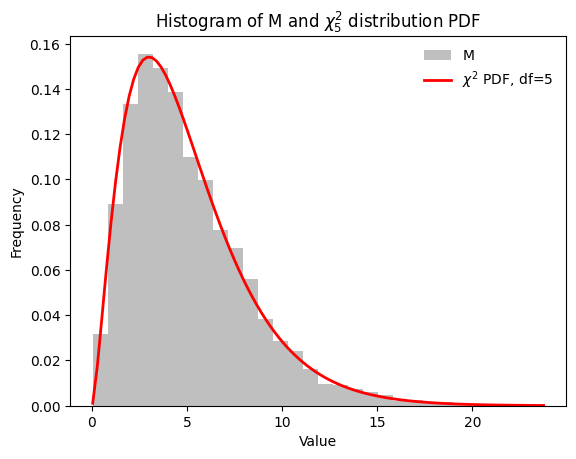
\includegraphics[height=6cm]{figures/chi-square.png}}
  \hspace{1cm}
  \subcaptionbox{$M$的Q-Q plot}%
                [7cm]{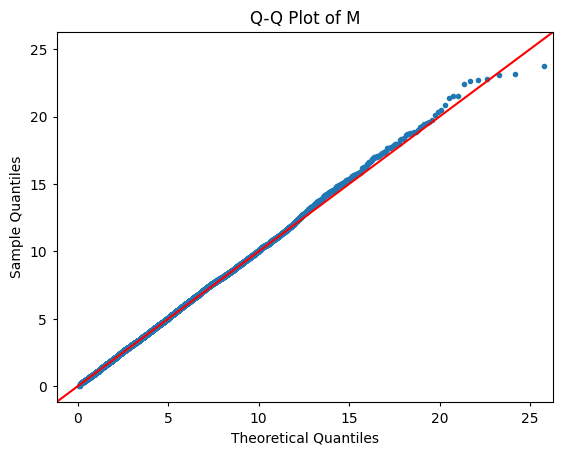
\includegraphics[height=6cm]{figures/qqplot.png}}
  \caption{$M$的渐进分布的数值模拟结果}
  \label{fig:bisubcaptionbox}
\end{figure}

如果样本量足够大,则我们可以提前指定$a$或$p_a$中的一个,然后利用定理\ref{theorem:M's distribution},$M \overset{d}\longrightarrow \chi^2_d$,求解出另一者。例如,在实际场景中,我们生成的$\mathbf{X}$的维数$d=5$,且要求重随机化的
可接受随机化的比例$P_a=80\%$,根据卡方分布的下80\%分位数结果得到$a=7.29$。

\subsubsection{平衡分组效应}

\begin{theorem}\label{theorem:covariance}\cite{morgan2012rerandomization}
    假定重随机化使用的准则为$\varphi_M$且$p_w=\frac{1}{2}$。若$\overline{\mathbf{X}}_T-\overline{\mathbf{X}}_C$服从多元正态分布,那么有
    \begin{equation}
        \operatorname{cov}\left(\overline{\mathbf{X}}_T-\overline{\mathbf{X}}_C \mid \mathbf{X}, \varphi_M=1\right)=v_a \operatorname{cov}\left(\overline{\mathbf{X}}_T-\overline{\mathbf{X}}_C \mid \mathbf{X}\right),
    \end{equation}
    其中
    \begin{equation}\label{def: va}
        v_a \equiv \frac{2}{d} \times \frac{\gamma(d / 2+1, a / 2)}{\gamma(d / 2, a / 2)}=\frac{P\left(\chi_{d+2}^2 \leq a\right)}{P\left(\chi_d^2 \leq a\right)}
    \end{equation}
    且 $\gamma$ 是不完全伽马函数(Incomplete Gamma Function): $\gamma(b, c) \equiv \int_0^c y^{b-1} e^{-y} d y$.
    
\end{theorem}

根据\ref{def: va}中$v_a$的定义,我们可以知道$0\leq v_a\leq 1$,再结合定理\ref{theorem:covariance}可以看出,重随机化减少了协变量均值差异的抽样方差,使得差异更加集中于0附近。我们定义\textbf{方差的百分比减少量}(the Percent Reduction in Variance),即重随机化减少每个协变量$\mathbf{x}_j$均值差异的方差的百分比:
\begin{equation}\label{varianceReduction}
100\left(\frac{\operatorname{var}\left(\bar{X}_{j, T}-\bar{X}_{j, C} \mid \mathbf{X}\right)-\operatorname{var}\left(\bar{X}_{j, T}-\bar{X}_{j, C} \mid \mathbf{X}, \varphi=1\right)}{\operatorname{var}\left(\bar{X}_{j, T}-\bar{X}_{j, C} \mid \mathbf{X}\right)}\right) .
\end{equation}

根据定理\ref{theorem:covariance}和定义\ref{varianceReduction},对于每个协变量,它的方差的百分比减少量为,
\begin{equation}
    100(1-v_a).
\end{equation}

\begin{figure}[!htbp]
    \centering
    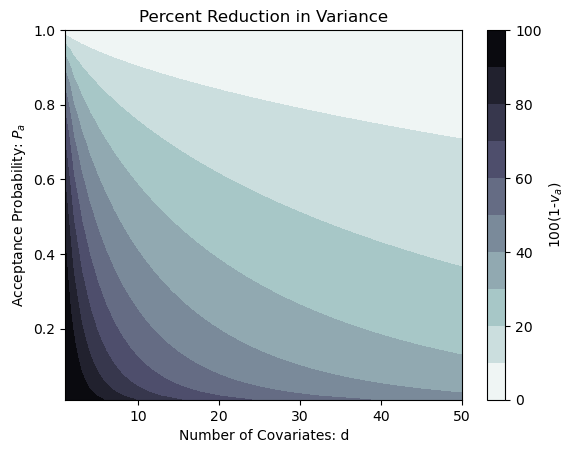
\includegraphics[width=0.55\linewidth]{figures/100(1-va).png}
    \caption{$\bar{X}_{T}-\bar{X}_{C}$的方差百分比减少量$100(1-v_a)$关于$d$和$P_a$的函数图像}
    \label{fig:100(1-va)}
\end{figure}

为了更加直观地展示方差的百分比减少量$100(1-v_a)$与协变量维数$d$和可接受随机化比例$P_a$的关系我们绘制了图\ref{fig:100(1-va)}。从图\ref{fig:100(1-va)}中我们可以发现,需要平衡的协变量维数$d$越小,可接受随机化比例$P_a$越接近0,协变量组间差异的均值的方差的百分比减少量$100(1-v_a)$越大。



\subsection{ATE的估计的准确性}

只要实验结果与协变量存在相关性,重随机化就能提高平均处理效应的估计$\hat{\tau}$的精度。因此,实验设计者可以仅仅以计算时间为代价,降低ATE的估计的方差,提升估计的准确性。

\begin{theorem}
    如果
    \begin{enumerate}
        \item 使用$\varphi_M$进行重随机化且$P_w=\frac{1}{2}$;
        \item 协变量$\mathbf{X}$和结果$\mathbf{Y}$均服从正态分布;
        \item 处理效应$\tau$是可加的,
    \end{enumerate}
    那么$\hat\tau$的方差的百分比减小量是
    \begin{equation}
        100(1-v_a)R^2,
    \end{equation}
    其中$R^2$表示在实验组内,结果$\mathbf{Y}$和协变量$\mathbf{X}$之间的多重相关系数的平方,而 $v_a$ 同定理\ref{theorem:covariance}中的定义一致。
\end{theorem}

\begin{figure}[!htbp]
    \centering
    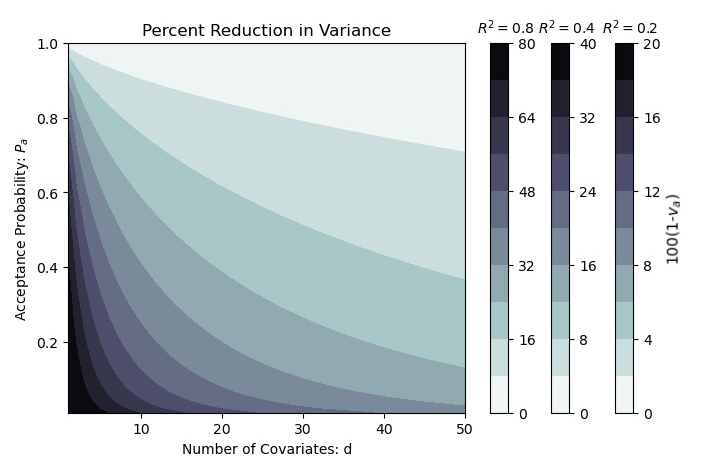
\includegraphics[width=0.68\linewidth]{figures/tau_percent_Reduction_in_Variance.png}
    \caption{$\hat\tau$的方差百分比减少量$100(1-v_a)$关于$d$、$P_a$和$R^2$的函数图像}
    \label{fig:tau_percent_Reduction_in_Variance}
\end{figure}

图\ref{fig:tau_percent_Reduction_in_Variance}所示的是平均处理效应的估计$\hat{\tau}$的方差百分比减少量关于$d$、$p_a$和$R^2$的函数图像。为了更好的可视化,此处选取了$R^2=0.8, 0.4, 0.2$,将$d$和$p_a$分别作为图像的横、纵坐标,绘制了图像。进一步地,我们可以发现,如果结果$\mathbf{Y}$和协变量$\mathbf{X}$之间的多重相关系数越大,平均处理效应的估计$\hat{\tau}$的方差百分比减少量越大。

\subsubsection{使用 Mahalanobis 距离的重随机化在高维数据下的挑战}

在统计学发展的大多数时间中,我们研究的每个样本上测量的特征数量相对较少,导致了传统理论和实践主要局限于“大样本量,小维数”的情形。近些年来,随着数据获取技术和计算设施的令人瞩目的发展,统计学研究的数据集中出现了许多数据量较少但是维度极大的情况,例如图像分析(image analysis),文本分类(document classification)与天文和大气科学等等\cite{johnstone2009statistical}。此时,许多传统的统计学习方法会面临维数灾难(Curse of Dimensionality)。使用 Mahalanobis 距离的重随机化也面临了高维数据的挑战,即如果$\mathbf{X}$的$\text{样本量}n <\text{维数}d$, 则使用可接受准则为$\varphi_M$的重随机化,无论如何选取分组结果$\mathbf{W}$,$M$都为确定的值。

我们对$100\times 200$的协变量矩阵$\mathbf{X}$进行了5000次随机平均分组,并计算了相应分组的Mahalanobis距离,进而绘制了Mahalanobis距离的频数直方图。如图\ref{fig:different Distance}(a)中对$M$的数值模拟结果所示,在高维的$\mathbf{X}$的情况下,准则$\varphi_M$会使得$M$失去随机性,从而导致重随机化失效。一旦设置好阈值$a$,无论如何选取$\mathbf{W}$, 重随机化只会一直接受或一直拒绝随机化分组。因此,在高维的场景下,实验设计者应当避免使用 Mahalanobis 距离参与重随机化。为此,实验设计者可以考虑使用欧氏距离即$\mathrm{l}_2$距离,类似于\ref{重随机化准则}构造相应的可接受随机化准则函数:
\begin{equation}
    D  \equiv\left(\overline{\mathbf{X}}_T-\overline{\mathbf{X}}_C\right)^{\top}\left(\overline{\mathbf{X}}_T-\overline{\mathbf{X}}_C\right). 
\end{equation}

\begin{figure}[!hbtp]
  \centering
  \subcaptionbox{$M$、$M_1$和$D$的频数直方图}%
                [7cm]{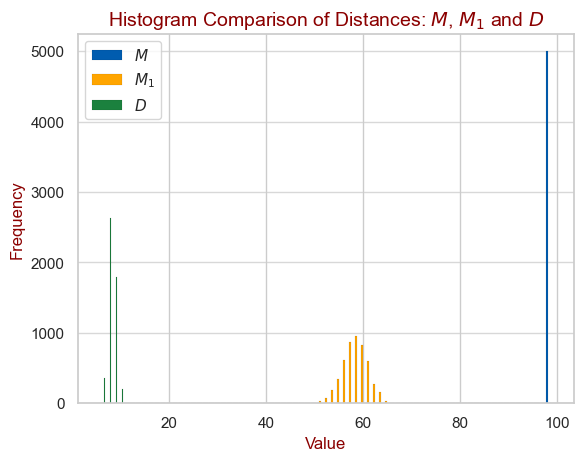
\includegraphics[height=6cm]{figures/differentDistance.png}}
  \hspace{1cm}
  \subcaptionbox{$M_{\lambda}$的均值和方差关于$\lambda$的折线图}%
                [7cm]{\includegraphics[height=6cm]{figures/Mahalanobis distance’s mean and variance.png}}
  \caption{$M$、$M_1$和$D$的数值模拟结果}
  \label{fig:different Distance}
\end{figure}

\begin{figure}[!htbp]
    \centering
    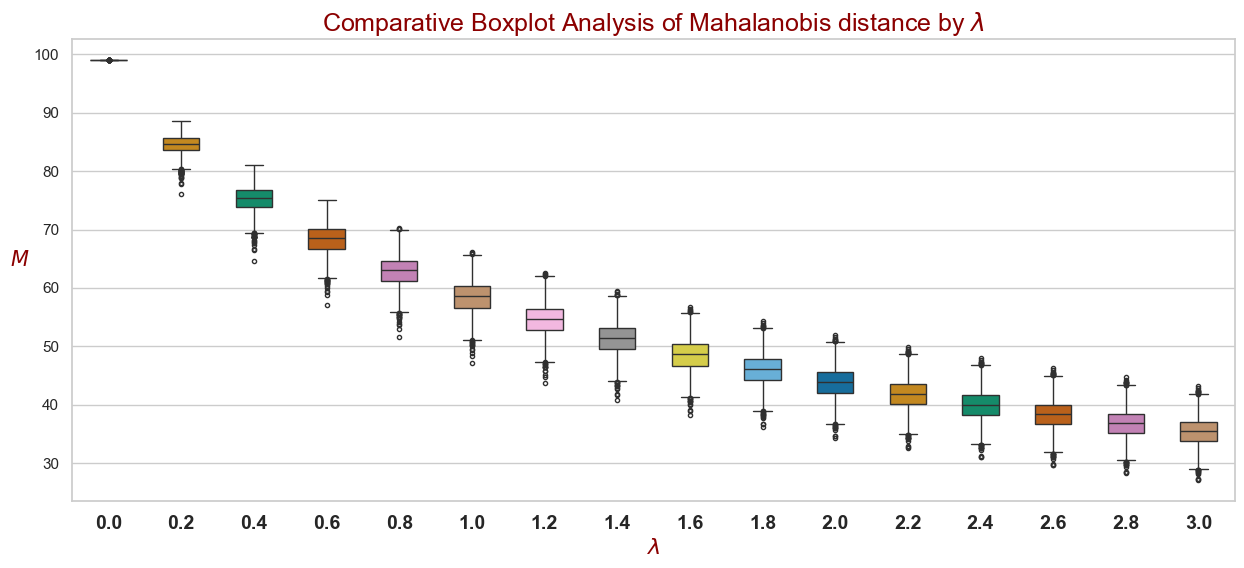
\includegraphics[width=1\linewidth]{figures/boxplot_Mahalanobis_distance_by_lambda.png}
    \caption{$M_{\lambda}$关于$\lambda$的箱线图}
    \label{fig:M_lambda's boxplot}
\end{figure}

或者,我们可以对使用Mahalanobis距离的可接受随机化函数进行一定的调整:加入正则化项$\lambda I_d$。在加入正则化项后的Mahalanobis距离具体表达式如下:
\begin{equation}
    M_{\lambda}=n p_w\left(1-p_w\right)\left(\overline{\mathbf{X}}_T-\overline{\mathbf{X}}_C\right)^{\top} \left(\operatorname{cov}(\mathbf{X})+\lambda I_d\right)^{-1}\left(\overline{\mathbf{X}}_T-\overline{\mathbf{X}}_C\right),\ \lambda > 0.
\end{equation}

如图\ref{fig:different Distance}(a)中$M_1$和$D$的频数直方图所示,无论是使用$\mathrm{l}_2$距离,还是对Mahalanobis距离加入正则化项,随着随机化产生了不同的分组结果$W$,组间距离都保持了随机性。从图\ref{fig:different Distance}(b)和图\ref{fig:M_lambda's boxplot}中可以看出,随着选取的$\lambda$的增大,随机化产生的$M_{\lambda}$的均值会减小。而$M_{\lambda}$的方差则呈现先上升后下降的趋势。由此可见,实验设计者应当避免选取过大的$\lambda$,以免出现$M_{\lambda}$的随机性不足的情况。

% \begin{theorem}\label{M's disadvantage}
%     假定重随机化使用的准则为$\varphi_M$且$P_w=\frac{1}{2}$。若对于$n\times d$的$\mathbf{x}$满足 $n < d$和$\operatorname{Rank}(\mathbf{x}) = n$,则对于任意分组$\mathbf{W}$, 有
%     $$
%     M \equiv \mathbb{1}_{T-C}^{\top}H^{-1}\mathbb{1}_{T-C}.
%     $$
%     其中,$\mathbb{1}_{T-C} = \mathbf{W} - (\mathbb{1} - \mathbf{W})$, $H = I_{n} - \frac{1}{n}\mathbb{1}_{n}\mathbb{1}_{n}^{\top}$。$\mathbb{1}_{n}$为$n$维全1列向量,$I_n$为$n\times n$的单位阵。
% \end{theorem}

% \begin{proof}
%     由定义\ref{x_T-x_C},
%     \begin{equation}
%         \overline{\mathbf{X}}_T-\overline{\mathbf{X}}_C=\frac{\mathbf{X}^{\top} \mathbf{W}}{n/2}-\frac{\mathbf{X}^{\top}(\mathbf{1}-\mathbf{W})}{n/2}=\frac{2}{n}\mathbf{X}^{\top}\mathbb{1}_{T-C} .
%     \end{equation}
%     根据定义\ref{M's def},
%     \begin{equation}\label{M in theorem 2.4}
%         \begin{aligned}
%             M & =n p_w\left(1-p_w\right)\left(\overline{\mathbf{X}}_T-\overline{\mathbf{X}}_C\right)^{\top} \operatorname{cov}(\mathbf{X})^{-1}\left(\overline{\mathbf{X}}_T-\overline{\mathbf{X}}_C\right)\\
%             & = \frac{1}{n}\mathbb{1}_{T-C}^{\top}\mathbf{X}\operatorname{cov}(\mathbf{X})^{-1}\mathbf{X}^{\top}\mathbb{1}_{T-C}.
%         \end{aligned}
%     \end{equation}
%     接下来关于样本均值$\bar{\mathbf{X}}$和样本方差$\operatorname{cov}(\mathbf{X})$做出一些推导,
%     \begin{equation}
%         \bar{\mathbf{X}} = \frac{1}{n}\sum_{i=1}^n \mathbf{X}_i = \frac{1}{n}\mathbf{X}^{\top}\mathbb{1}_n,
%     \end{equation}
%     \begin{equation}
%         HH^{\top} = (I_{n} - \frac{1}{n}\mathbb{1}_{n}\mathbb{1}_{n}^{\top})(I_{n} - \frac{1}{n}\mathbb{1}_{n}\mathbb{1}_{n}^{\top})^T = H,
%     \end{equation}
%     \begin{equation}\label{cov(X)}
%         \begin{aligned}
%              \operatorname{cov}(\mathbf{X})&=\frac{1}{n} \sum_{i=1}^n\left(\mathbf{x}_i-\bar{\mathbf{X}}\right)\left(\mathbf{x}_i-\bar{\mathbf{X}}\right)^T\\
%             &= \frac{1}{n}\left(\mathbf{x}_1-\bar{\mathbf{X}},\cdots, \mathbf{X}_n-\bar{\mathbf{X}}\right)\left(\mathbf{x}_1-\bar{\mathbf{x}},\cdots, \mathbf{x}_n-\bar{\mathbf{x}}\right)^T\\
%             &= \frac{1}{n} \left(\mathbf{X}^{\top} - \bar{\mathbf{X}}\mathbb{1}_{n}^{\top}\right)\left(\mathbf{X}^{\top} - \bar{\mathbf{X}}\mathbb{1}_{n}^{\top}\right)^{\top}\\
%             &= \frac{1}{n} \left(\mathbf{X}^{\top} - \mathbf{X}^{\top}\mathbb{1}_{n}\mathbb{1}_{n}^{\top}\right)\left(\mathbf{X}^{\top} - \mathbf{X}^{\top}\mathbb{1}_{n}\mathbb{1}_{n}^{\top}\right)^{\top}\\
%             & = \frac{1}{n}\mathbf{X}^{\top}(I_{n} - \frac{1}{n}\mathbb{1}_{n}\mathbb{1}_{n}^{\top})(I_{n} - \frac{1}{n}\mathbb{1}_{n}\mathbb{1}_{n}^{\top})^{\top}\mathbf{X}\\
%             & = \frac{1}{n}\mathbf{X}^{\top}HH^{T}\mathbf{X}\\
%             & = \frac{1}{n}\mathbf{X}^{\top}H\mathbf{X}.
%         \end{aligned}
%     \end{equation}
%     对$\mathbf{X}$进行SVD分解,
%         \begin{equation}\label{SVD}
%             \mathbf{X} = U \Sigma V^{\top},
%         \end{equation}
%     其中$U$为$n\times n$的矩阵,$\Sigma$为$n\times n$的对角矩阵,$V$为$n\times d$的矩阵。
    
%     由于$\operatorname{Rank}(\mathbf{X})=m$,$U$为正交矩阵,满足
%     \begin{equation}
%         U^{\top}U=UU^{\top}=I_n. 
%     \end{equation}
%     将\ref{SVD}代回\ref{cov(X)},
%     \begin{equation}\label{cov(X)_1}
%         \begin{aligned}
%             \operatorname{cov}(\mathbf{X}) &= \frac{1}{n}V \Sigma U^{\top} H U \Sigma V^{\top}.\\
%         \end{aligned}
%     \end{equation}
%     将\ref{SVD}和\ref{cov(X)_1}代回\ref{M in theorem 2.4},
%     \begin{equation}
%         \begin{aligned}
%             M &= \mathbb{1}_{T-C}^{\top}U \Sigma V^{\top}(V \Sigma U^{\top} H U \Sigma V^{\top})^{-1}V \Sigma U^{\top}\mathbb{1}_{T-C}\\
%             &= \mathbb{1}_{T-C}^{\top}H\mathbb{1}_{T-C}.\\
%         \end{aligned}
%     \end{equation}
%     由$\mathbb{1}_{T-C} = \mathbf{W} - (\mathbb{1} - \mathbf{W})=2\mathbf{W}-\mathbb{1}$,
%     \begin{equation}
%         \begin{aligned}
%             M &= \mathbb{1}_{T-C}^{\top}H\mathbb{1}_{T-C}\\
%             &= (2\mathbf{W}-\mathbb{1})^{\top}H(2\mathbf{W}-\mathbb{1})\\
%             &= 4\mathbf{W}^{\top}H\mathbf{W}-4\mathbf{W}^{\top}H\mathbb{1}+\mathbb{1}^{\top}H\mathbb{1}.
%         \end{aligned}
%     \end{equation}
%     $H$是对角线元素相同且除对角线外其余元素也相同的$n\times n$方阵,故$M$不会随着$\mathbf{W}$的变化而变化。
    
% \end{proof}

% 由\ref{M's disadvantage}可知,

% 论文正文是主体,一般由标题、文字叙述、图、表格和公式等部分构成 \cite{Yang1999}。一般可包括理论分析、计算方法、实验装置和测试方法,经过整理加工的实验结果分析和讨论,与理论计算结果的比较以及本研究方法与已有研究方法的比较等,因学科性质不同可有所变化。
% \par 论文内容一般应由十个主要部分组成,依次为:1.封面,2.中文摘要,3.英文摘要,4.目录,5.符号说明,6.论文正文,7.参考文献,8.附录,9.致谢,10.攻读学位期间发表的学术论文目录\cite{Yu2012}。
% \par 以上各部分独立为一部分,每部分应从新的一页开始,且纸质论文应装订在论文的右侧。


% \section{字数要求}
% \subsection{本科论文要求}
% 各学科和学院自定。理工科研究类论文一般不少于2万字,设计类一般不少于1.5万字;医科、文科类论文一般不少于1万字。

\section{本章小结}

随机化可以在组之间平衡协变量,但这只是平均意义上的,在任何一个实验中,协变量分组之间可能存在不平衡的现象。重随机化提供了一种简单直观的方法,以改善随机对照试验的协变量平衡。要执行重随机化,需要预先确定一个随机化是否可接受的准则。为了保证无偏性,这个规则需要保证实验组和对照组的受试者数量的均衡。本章证明了给定协变量矩阵,在大样本的情况下,实验组和对照组间的Mahalanobis距离服从自由度为协变量维数的卡方分布。如果采取的标准是每当Mahalanobis距离超过某个阈值时就重随机化,那么重随机化可以降低两组间均值差异的方差,且当协变量与结果相关时,重随机化会增加处理效应估计的精确度。在面临高维数据时,使用Mahalanobis距离的重随机化会失去随机性。为了解决以上问题,实验设计者可以考虑使用其他方式构造可接受随机化准则函数。
